\section{Model families and blending}
\label{sec:families}

Once single-model capacity is exhausted, the only remaining mechanism with a plausible sign is
to combine models whose errors are not the same. We therefore trained nine members under the
same folds and transforms: LightGBM with the adopted target statistics, four other boosted
configurations (XGBoost, CatBoost with 2{,}500 GPU iterations and native categorical handling,
LightGBM with linear leaves, LightGBM with DART dropout), two multilayer perceptrons (one on the
raw frame with embeddings, one on the 33 encoded numeric features), an FT-Transformer
\citep{gorishniy2021}, and --- as a deliberately different information source --- a model trained
only on the 129{,}880 original survey rows.

\paragraph{The FT-Transformer.} Each feature becomes a token: an embedding for each of the 17
discrete fields (including the 3{,}474-level flight distance), a linear projection for each of
the four continuous fields, and a two-level embedding for the arrival-delay missing flag.
A learnable class token is prepended and three pre-normalised transformer blocks
($d=64$, four heads, FFN width 128, dropout 0.1) process the 23 tokens; a linear head on the
class token outputs the logit. Training uses AdamW and a one-cycle schedule for 20 epochs at
batch 4{,}096, which costs 97 seconds per fold on a laptop GPU --- cheap enough for five folds
in eight minutes.

\paragraph{Weights follow decorrelation, not strength.} Figure~\ref{fig:members} shows the two
quantities that matter for a member: its own score and the correlation of its residuals with
the LightGBM member. Fitting non-negative weights that sum to one on the logits
(Section~\ref{sec:stacking}) gives the lower panel. The best single model, LightGBM, ends up
with weight 0.012, while CatBoost (0.207), \texttt{linear\_tree} (0.179), XGBoost (0.155) and
the FT-Transformer (0.249) carry the ensemble. The FT-Transformer is the clearest case: it is
$2.0\times10^{-3}$ weaker than LightGBM alone and yet takes the largest weight, because it is
the most different strong member.

\begin{figure}[t]
\centering
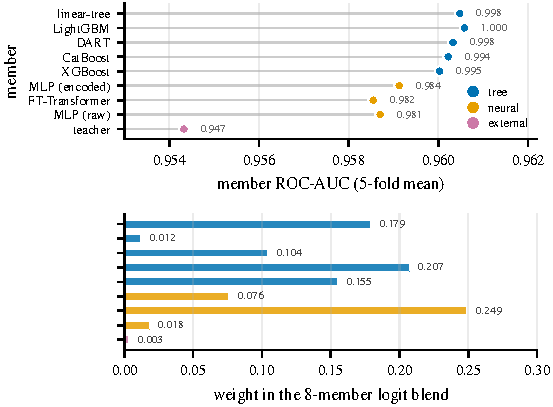
\includegraphics[width=0.68\linewidth]{figures/fig_members.pdf}
\caption{Members of the eight-family blend. Top: five-fold mean \auc{} with the residual
correlation against LightGBM printed next to each point. Bottom: weight fitted on the logits.
Strength and weight are almost independent: the two MLPs and the FT-Transformer absorb the
weight that the boosted trees cannot supply.}
\label{fig:members}
\end{figure}

Table~\ref{tab:blends} traces the ensemble. Three families (LightGBM, XGBoost, MLP) add
\dlt{1.07} over the multi-seed single model; five more members \dlt{1.0}; the FT-Transformer
another \dlt{1.0}. Each of these steps is at the noise floor on its own, but they are
\emph{cumulative} and each is confirmed by the leaderboard, which is the point of
Section~\ref{sec:lb}.

\begin{table}[t]
\centering
\small
\caption{Ensemble ladder. ``Public'' is the leaderboard score of the submitted file; the
transfer column is $\Delta$public$/\Delta$CV for that step.}
\label{tab:blends}
\begin{tabular}{lcccccc}
\toprule
Configuration & CV & OOF & public & rank & $\Delta$CV (\dlt{}) & transfer\\
\midrule
5 folds $\times$ 1 seed                & 0.960533 & 0.960526 & 0.96027 & 1331/2977 & --- & ---\\
5 folds $\times$ 3 seeds               & 0.960589 & 0.960580 & 0.96028 & 1340/2991 & $+0.55$ & 0.18\\
3 families (LGB+XGB+MLP)               & 0.960696 & 0.960688 & 0.96034 & 1307/3000 & $+1.07$ & 0.56\\
7 families                             & 0.960800 & 0.960793 & 0.96047 & 1254/3013 & $+1.04$ & 1.25\\
8 families ($+$FT-Transformer)          & 0.960901 & 0.960891 & \textbf{0.96062} & \textbf{1204/3061} & $+1.00$ & 1.50\\
8 families ($+$FT$\times$3 seeds)      & \textbf{0.960942} & 0.960932 & 0.96061 & --- & $+0.42$ & $-0.02$\\
\bottomrule
\end{tabular}
\end{table}



\section{What does not work}
\label{sec:rejected}

Figure~\ref{fig:ablation} collects the interventions that attribute to a single change, with
their measured effect. The lower half of the list is as informative as the upper half.

\paragraph{Variance control.} Averaging three seeds per fold buys \dlt{0.55} in CV and
\dlt{0.1} on the leaderboard. Ten folds instead of five buys \dlt{0.14} cross-validated: the
probe in Table~\ref{tab:protocol} shows that training each model on 72\% instead of 64\% of the
data helps, but the extra averaging over ten models cancels it (10 folds $\times$ 3 seeds:
0.961355; 5 folds $\times$ 3 seeds: 0.961356 on the same probe split). Strengthening the best
member behaves the same way: three seeds lift the FT-Transformer from 0.958548 to 0.959258 and
the blend from 0.960901 to 0.960942, yet the public score moves from 0.96062 to 0.96061.

\begin{table}[t]
\centering
\small
\caption{Protocol probe on a fixed 20\% split (139{,}927 rows): the dev part is re-split into
$k$ folds, each model is trained on $k-1$ of them and the predictions are averaged before
scoring. ``Train fraction'' is relative to the full training file.}
\label{tab:protocol}
\begin{tabular}{lcccc}
\toprule
Configuration & train fraction & probe \auc{} & $\Delta$ (\dlt{}) & time\\
\midrule
5 folds $\times$ 1 seed   & 0.64 & 0.961305 & --- & 47 s\\
5 folds $\times$ 3 seeds  & 0.64 & 0.961356 & $+0.55$ & 96 s\\
10 folds $\times$ 1 seed  & 0.72 & 0.961319 & $+0.14$ & 106 s\\
10 folds $\times$ 3 seeds & 0.72 & 0.961355 & $+0.50$ & 211 s\\
\bottomrule
\end{tabular}
\end{table}

\paragraph{Stacking.}
\label{sec:stacking}
We tried five meta-learners on the member logits, all cross-fitted (fit on four folds, predict
the held-out one): logistic regression with four values of $C$, a LightGBM meta-model on the
seven logits, the same plus member-disagreement features, the same plus the 21 raw features
(conditional stacking), and one weight vector per cabin$\times$travel segment. None of them
beats the fixed mean-weight blend (Table~\ref{tab:stacking}). The reason is visible in
Figure~\ref{fig:members}: with residual correlations between 0.977 and 1.000 the meta-model has
nothing to learn except a global reweighting, and the fitted weights already do that. A
meta-model can only pay when the members are both strong and genuinely different.

\begin{table}[t]
\centering
\small
\caption{Cross-fitted stacking against the fixed-weight blend (0.960800). ``$z$'' is the paired
DeLong statistic; every value is statistically indistinguishable from zero.}
\label{tab:stacking}
\begin{tabular}{lcccc}
\toprule
Meta-learner & fold mean & $\Delta$ (\dlt{}) & folds ahead & $z$\\
\midrule
Logistic on logits ($C=0.01$--$10$)   & 0.960797 & $-0.04$ & 1/5 & $-0.6$\\
LightGBM on 7 logits                  & 0.960799 & $-0.01$ & 3/5 & $-0.3$\\
LightGBM on logits $+$ spread         & 0.960826 & $+0.26$ & 4/5 & $-0.2$\\
LightGBM on logits $+$ raw features   & 0.960811 & $+0.11$ & 3/5 & $-0.2$\\
Per-segment weight vectors (6)        & 0.960810 & $+0.09$ & 3/5 & $+0.1$\\
\bottomrule
\end{tabular}
\end{table}

\paragraph{Feature-side variants.} Multi-view auxiliary features (three LightGBMs trained on
feature subsets, their cross-fitted logits appended) give \dlt{0.57} at $p=0.81$ and three of
five folds: rejected. Pseudo-labelling the 6.6\% of test rows the blend is confident about
produces a member at 0.960549 with residual correlation 0.9994 --- worse than the plain
LightGBM it was meant to help. A target encoding of the full 17-column signature, extra
distance-segment encodings and \texttt{max\_bin}$=4095$ are all at or below zero.

\paragraph{Weak but different is not enough.} The teacher trained only on the original survey is
the most decorrelated member we found (residual correlation 0.947, against 0.981 for the best
MLP) and it is worthless: at 0.954326 its fitted weight is 0.003. Contribution requires
\emph{both} properties --- a member needs to be within about $2\times10^{-3}$ of the leader and
have a residual correlation below roughly 0.99. Finally, PyTabKit's RealMLP with default
hyper-parameters \citep{holzmuller2024} trained for 30 epochs costs 6.9 minutes per fold and
reaches only 0.958281, so we did not include it; the published recipe relies on an ensemble of
many seeds, which is the family-level move we already exploit through the FT-Transformer.

\begin{figure}[t]
\centering
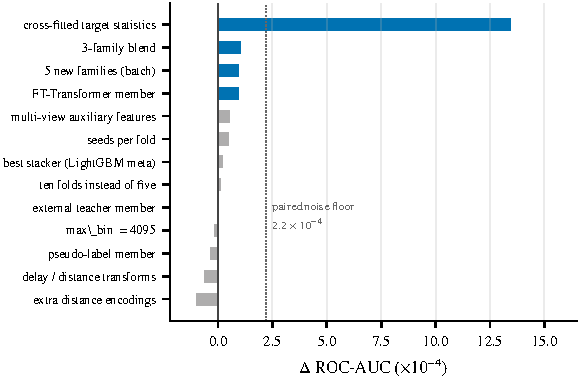
\includegraphics[width=0.68\linewidth]{figures/fig_ablation.pdf}
\caption{Every intervention measured against the same reference, in units of \dlt{}.
Blue: adopted. Grey: measured and rejected. The dotted line is the paired noise floor
(\dlt{2.2}); everything to its left is indistinguishable from retraining with another seed.}
\label{fig:ablation}
\end{figure}
